% !TEX root = ../main.tex
\pagebreak[0]
\section{\emph{Arc} configurations}\label{sec:arc-configurations}

\begin{figure}[htbp]
\centering
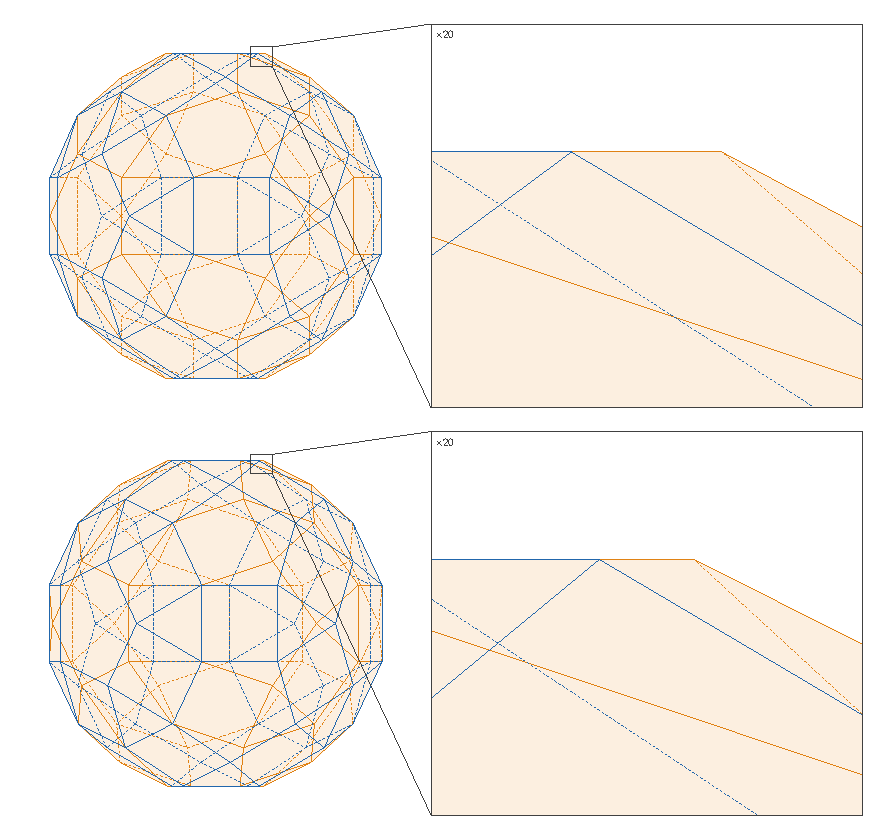
\includegraphics[width=\linewidth]{figures/arcs}
\caption{Two touch configurations on the first arc of the plane $\Pi_1$, at $e=1/10$ and $e=3/20$ ($t=0$, $\theta=0$); the \fc{Hole}{hole (orange)} and the \fc{Plug}{plug (blue)} as in \cref{fig:global-examples}. Both shadows reach exactly as far in the upward screen direction, which is $\mathbf e_2$, and share their top edge. The enlargements, $20$ times at the right ends of the two top edges, show the plug's top edge ending inside the hole's.}
\label{fig:arc-examples}
\end{figure}

The boxes left unresolved by the preceding components cluster around
configurations with $t=0$, a range of values of $s$, and a relative
rotation close to a turn through $36^\circ$ about a five-fold axis of the
RID, followed by a small turn about the second coordinate axis. For $t=0$,
that axis lies in the shadow plane, and a turn about it does not change
how far the plug reaches in its direction. The $36^\circ$ turn happens to
leave that reach equal to the hole's, so whatever the second turn, the
plug's shadow reaches exactly as far as the hole's in that direction, and
none of these configurations is a fit. This gives two planes of configurations, each a
no-fit set for a reason as simple as for the aligned configurations. Around
the touch configurations in them, the Exotic component uses tube
zooms that divide out the distance from such a plane, much as the Local
component divides out the size of the rotation.

\subsection{Geometry of \emph{non-aligned touch} configurations}\label{subsec:geometry-of-non-aligned-touch-configurations}

\paragraph{The arc planes.}
Let
\[
  a_1=\frac{-5+3\sqrt5}{10},\qquad a_3=\frac{-5+\sqrt5}{10},\qquad
  \mathbf r_A=(a_1,0,a_3),
\]
and, for $\sigma\in\{-1,1\}$, $\mathbf w_\sigma=(\sigma a_3,1,-\sigma a_1)$.
The two \emph{arc planes} are the families of configurations
\begin{equation}\label{eq:arc-plane}
  \Pi_\sigma=\bigl\{[s,0,\sigma\mathbf r_A+\theta\mathbf w_\sigma]:\ s,\theta\in\mathbb R\bigr\},
  \qquad \sigma\in\{-1,1\},
\end{equation}
two-dimensional sets of configurations with $t=0$. Since
$\lVert\mathbf r_A\rVert=\tan18^\circ$, the rotation $R_P(\mathbf r_A)$ is a turn
through $36^\circ$ about the axis of $\mathbf r_A$, which is a five-fold axis
of the RID; its square is a symmetry of $\mathcal R$, but it is not one
itself. With $\mathbf e_2=(0,1,0)$, the quaternion product gives
\[
  (1,\theta\mathbf e_2)(1,\sigma\mathbf r_A)
  =(1-\theta\sigma\,\mathbf e_2\cdot\mathbf r_A,\ \theta\mathbf e_2+\sigma\mathbf r_A
     +\theta\sigma\,\mathbf e_2\times\mathbf r_A)
  =(1,\sigma\mathbf r_A+\theta\mathbf w_\sigma),
\]
because the second coordinate of $\mathbf r_A$ is zero. Hence
$R_P(\sigma\mathbf r_A+\theta\mathbf w_\sigma)=R_P(\theta\mathbf e_2)R_P(\sigma\mathbf r_A)$:
the plug is first turned through $36^\circ$ and then through the angle
$2\arctan\theta$ about the second coordinate axis.

\begin{lemma}[The arc planes contain no fit]\label{lem:arc-planes-contain-no-fit}
  No configuration in $\Pi_{1}$ or $\Pi_{-1}$ is a fit.
\end{lemma}
\begin{proof}
  On $\Pi_\sigma$ we have $t=0$, so $\mathbf e_2$ is perpendicular to
  $\mathbf u=(s,0,1)$: it is a direction in the shadow plane, and
  $\mathbf e_2\cdot\mathbf x$ is unchanged by projection. A turn about the
  second coordinate axis does not change $\mathbf e_2\cdot\mathbf x$ either.
  So the plug's support value in the direction $\mathbf e_2$ is
  \[
    \max_{\mathbf v\in V}\mathbf e_2\cdot R_P(\sigma\mathbf r_A)\mathbf v
     =2+\sqrt5=\max_{\mathbf v\in V}\mathbf e_2\cdot\mathbf v,
  \]
  the hole's support value; the middle equality is an exact comparison over
  the sixty vertices of \cref{eq:rhombicosidodecahedron-vertices}. A fit
  places the compact plug shadow in the interior of the hole shadow, which
  requires a strictly smaller support value in every direction of the
  shadow plane.
\end{proof}

The two planes describe the same plug positions, since
$R_P(\mathbf r_A)^2$ is a symmetry of the plug, but they are different
subsets of $B_0$. Both lie in the hyperplanes on which the following
inequalities hold with equality, so their configurations in $D$ lie on the
boundary of $D$: on $\Pi_\sigma$, the
relative-rotation comparison
\begin{equation}\label{eq:tie-inequality}
  \sigma\bigl(\varphi^{-1}r_1-r_3\bigr)\le2-\varphi
\end{equation}
of \cref{eq:reduced-domain} (the one with $i=3$, $\epsilon=-\sigma$ and
$\delta=\sigma$) holds with equality, because
$\varphi^{-1}a_1-a_3=2-\varphi$ and $a_1+\varphi^{-1}a_3=0$. Along the plane,
two representatives of the same configuration tie, and the comparison
decides between them; we call \cref{eq:tie-inequality} the \emph{tie
inequality} of $\Pi_\sigma$. Every construction below comes in two copies,
one for each sign $\sigma$; the map $(r_1,r_2,r_3)\mapsto(-r_1,r_2,-r_3)$
exchanges the two planes, keeping $s$ and $\theta$, together with their tie
inequalities.

\paragraph{Arc coordinates.}
Near $\Pi_\sigma$ we use the coordinates
\begin{equation}\label{eq:arc-coordinates}
  e=\frac{1-2s}{2+s},\quad v=\frac{5t}{2+s},\quad \theta=r_2,\quad
  \zeta_1=r_1-\sigma(a_1+a_3\theta),\quad
  \zeta_3=r_3-\sigma(a_3-a_1\theta),
\end{equation}
defined for $s>-2$. Then
\[
  \mathbf u=(1-2e,\ v,\ 2+e)=\frac5{2+s}(s,t,1),\qquad
  \mathbf r=\sigma\mathbf r_A+\theta\mathbf w_\sigma+(\zeta_1,0,\zeta_3),
\]
so $\mathbf u$ is a positive multiple of $(s,t,1)$ with components affine
in $e$ and $v$, as zooms require, and every witness is again a polynomial
in the new coordinates. The plane $\Pi_\sigma$ is $v=\zeta_1=\zeta_3=0$. The
coordinate $e$ is chosen so that both families of touch configurations
below are straight lines in the plane, crossing at $e=0$; this matters for
the shear in \cref{subsec:eliminating-the-crossing-configuration}.

\paragraph{The arcs.}
Inside each plane lie two segments of touch configurations
(\cref{fig:arc-examples,fig:endpoint-crossing-examples}):
\begin{itemize}
  \item the \emph{first arc}, $\theta=0$ with $0\le e\le e_*=\sqrt5-2$, that is
    $s\in[\sqrt5-2,1/2]$;
  \item the \emph{second arc}, $\theta=-e$ with $0\le e\le e_*$.
\end{itemize}
Along the first arc, the two shadows share their top edge in the direction
$\mathbf e_2$, the plug's top edge ends inside the hole's, and the rest of
the plug's shadow lies inside the hole's. At the \emph{endpoint} $e=e_*$, the
ends of the two top edges coincide; beyond it, the plug's top edge is the
longer one, and its corner pokes out. The two arcs meet at the
\emph{crossing}, $e=0$, where $s=1/2$. Elsewhere in the plane, the
configurations are poke configurations, and the Global component handles
them (\cref{fig:arc-plane-slice}). These properties explain where zooms are
needed; the proof itself uses only \cref{lem:arc-planes-contain-no-fit}.

The second arc lies outside $D$ except at the crossing. On it, the
polynomial of one of the fold inequalities of \cref{eq:reduced-domain},
written homogeneously in the viewing vector $(1-2e,v,2+e)$, equals
$5e^2+5e^4$, which is positive for $e>0$. Sufficiently small boxes around
its configurations with $e>0$ are therefore eliminated by the Domain
component, and no cover follows the second arc; near the crossing it is
handled in \cref{sec:endpoint-and-crossing-configurations}.

\begin{figure}[htbp]
\centering
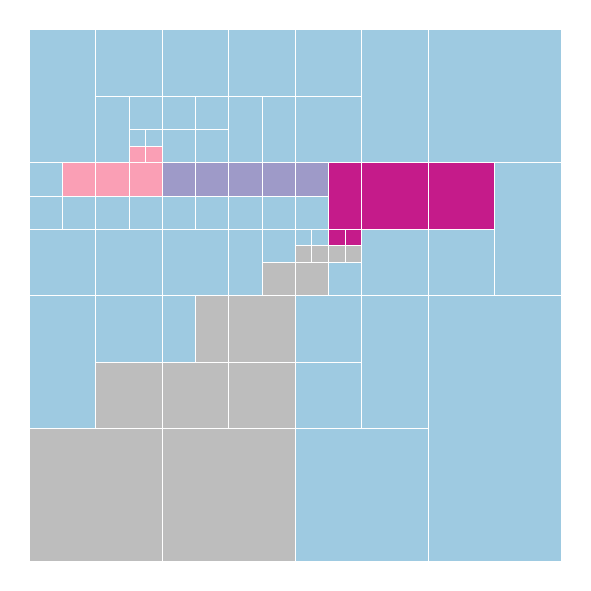
\includegraphics[width=0.55\linewidth]{figures/slice-arcs}
\caption{A slice of the final collection through the plane $\Pi_1$: horizontally $s\in[3/16,5/8]$, vertically $\theta\in[-5/16,1/8]$ (with $\mathbf r_A$ rounded to rationals within $10^{-14}$), halved alternately until one component eliminates each piece, which is coloured by that component: \fc{Global}{light blue Global}, \fc{Domain}{grey Domain}, \fc{Arc}{lavender the arc cover}, \fc{Endpoint}{light pink the endpoint cover} (near $s=\sqrt5-2$) and \fc{Crossing}{magenta the crossing cover} (near $s=1/2$). The first arc is the segment $\theta=0$ between these two values. The Global component handles the configurations of the plane away from the arcs, and the Domain component the pieces outside $D$, including those along the second arc away from the crossing.}
\label{fig:arc-plane-slice}
\end{figure}

\subsection{Eliminating \emph{arc} configurations}\label{subsec:eliminating-arc-configurations}

Along the first arc, a small displacement off the plane $\Pi_\sigma$ moves
some projected plug vertex beyond the hole shadow at a rate proportional to
the displacement. This is the situation of the aligned configurations, and
the tube zooms of \cref{subsec:the-zoom-lemma} apply.

\paragraph{The arc covers.}
Along the first arc of $\Pi_\sigma$, the base coordinate is $e$ and the
offset coordinates are $(v/2,\theta,\zeta_1,\zeta_3)$, weighting $v$ by one
half. The offset box is $\Phi=[0,1]\times{[-1,1]}^3$, since $t\ge0$ forces
$v\ge0$. This gives seven tube zooms, with $e\in[3/64,3/16]$ and
$\delta_{\max}=1/32$, so the covered set consists of the configurations with
\[
  \frac3{64}\le e\le\frac3{16},\qquad 0\le v\le\frac1{16},\qquad
  |\theta|,|\zeta_1|,|\zeta_3|\le\frac1{32}.
\]
The no-fit set of the zooms is the plane $\Pi_\sigma$: where $\delta=0$, the
offsets vanish, so the configuration lies on the first arc. The view
$\mathbf u=(1-2e,v,2+e)$ has $u_3=2+e>0$ and components affine in each zoom
coordinate, as \cref{def:zoom} requires. The weight of $v$, the radii and
the range of $e$ are tuning choices: the proof needs only that every cell
passes its check and that the covers overlap as described in
\cref{subsec:the-arcs-together}.

Most cells carry gap polynomials with the zoom factor $\delta$. Part of the
covered set lies on the far side of the tie inequality, outside $D$; there
the tie inequality itself serves as the witness. The cover for $\sigma=1$
has 343 terminal cells, 32 of them with the tie inequality, and the cover
for $\sigma=-1$ has 288, with 72.

\begin{proposition}[The arc neighbourhoods]\label{prop:arc-neighbourhoods}
  For each $\sigma\in\{-1,1\}$, no configuration of $D$ in the covered set
  above is a fit.
\end{proposition}
\begin{proof}
  By \cref{lem:tube-coverage}, such a configuration lies in
  $\Pi_\sigma$, which contains no fit by
  \cref{lem:arc-planes-contain-no-fit}, or in a checked cell. There
  \cref{lem:zoom-lemma} applies to the cell's witness: a gap polynomial
  excludes a fit, and the tie inequality shows that the configuration lies
  outside $D$.
\end{proof}

A search box lies in the covered set exactly when the ranges of the five
arc coordinates over the box lie in the stated intervals. The coordinates
$e$ and $v$ are monotone in $s$ and in $t$ separately, and $\theta$,
$\zeta_1$ and $\zeta_3$ are affine in $\mathbf r$, so each range is attained at
corners of the box and the inclusion test consists of exact comparisons.

\paragraph{Where the arc covers stop.}
The arc covers stop short of both $e=0$ and $e=e_*$. The rate at which a
displacement off the plane moves some projected vertex outward shrinks
linearly towards both ends of the first arc, like $e$ at the crossing and
like $e_*-e$ at the endpoint. At those two points the quotient after
dividing by $\delta$ vanishes in some directions, exactly as at the square
and pentagon configurations, and the unresolved boxes concentrate there
(\cref{fig:arcs-residual}). We treat the endpoint and the crossing with
point zooms in \cref{sec:endpoint-and-crossing-configurations}.

\begin{figure}[htbp]
\centering
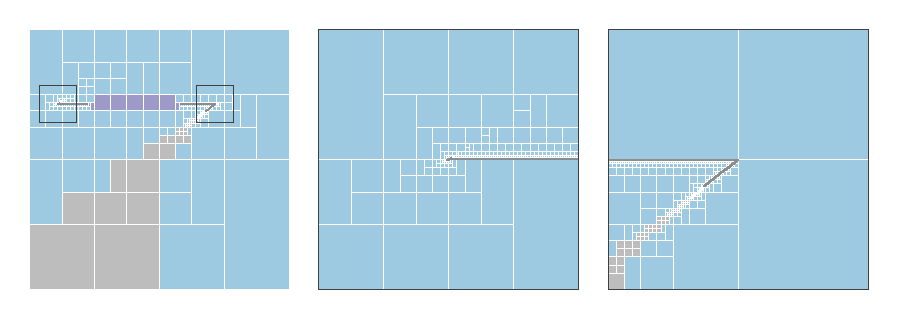
\includegraphics[width=\linewidth]{figures/arcs-residual}
\caption{The plane $\Pi_1$ as in \cref{fig:arc-plane-slice}, halved $18$ times with \fc{Arc}{the arc covers added (lavender)} but not yet the endpoint and crossing covers. Unresolved pieces (black) remain only near the two ends of the first arc. Middle: the window of half-width $1/32$ around the endpoint, $s=\sqrt5-2$, $\theta=0$; right: the same around the crossing, $s=1/2$, $\theta=0$, where the second arc leaves the first. Away from the crossing, the second arc lies outside $D$ \fc{Domain}{(grey)}.}
\label{fig:arcs-residual}
\end{figure}
